\section{Hilti Auspressgerät}
\label{Kapitel:Auspressgeraet}
Die von Hilti hergestellten chemischen Dübel bestehen aus zwei Komponenten. Diese werden bei der Anwendung gemischt und in ein vorgebohrtes Loch gedrückt. Durch das Mischen der Komponenten beginnt der Mörtel auszuhärten und befestigt dadurch eine ebenfalls in das Loch eingeführte Gewindestange.

Die Mörtelkomponenten werden mit einem eigens dafür entwickelten Auspressgerät in die Löcher gedrückt. Dieses Auspressgerät soll gleichzeitig möglichst zuverlässig und stabil sein, aber auch so konstruiert dass für die Anwendung wenig Kraft gebraucht wird und exakt so viel Fluid ausgepresst wird wie vom Anwender gewollt.\\
Das derzeit auf dem Markt erhältliche Gerät ist in Abbildung \ref{fig:Auspressgeraet} gezeigt.
%
\begin{figure}
    \centering
    \subfloat[Handgerät]{
        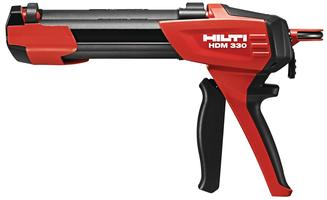
\includegraphics[width=0.31\textwidth]{figures/Auspressgeraet.jpg}
        \label{fig:Auspressgeraet:subA}
    }
    \subfloat[Akkugerät]{
        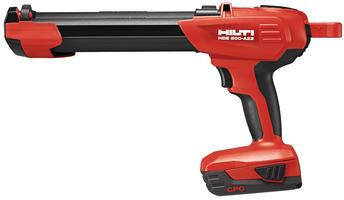
\includegraphics[width=0.31\textwidth]{figures/AuspressgeraetAkku.jpg}
        \label{fig:Auspressgeraet:subB}
    } 
    \subfloat[Mörtel Kartusche]{
        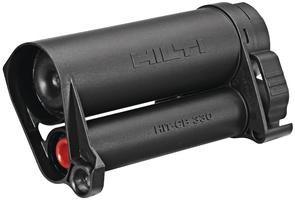
\includegraphics[width=0.31\textwidth]{figures/AuspressgeraetKasette.jpg}
        \label{fig:Auspressgeraet:subC}
    }
    \caption{Das Gerät zum Auspressen von Hilti Injektionsmörtel.\\In \subref{fig:Auspressgeraet:subA} ist das Handgerät zu sehen, in \subref{fig:Auspressgeraet:subB} die Ausführung mit Akku, bei der das Auspressen auf Knopfdruck geschieht.\\
    In \subref{fig:Auspressgeraet:subC} ist eine Kartusche abgebildet, in die die Mörtelbeutel gelegt werden.}
    \label{fig:Auspressgeraet}
\end{figure}
%

Das Mischen der beiden Komponenten geschieht in einem Mischer, der vorne am Auspressgerät angeschraubt wird (Abbildung \ref{fig:Mischer}).
%
\begin{figure}
    \centering
    \subfloat[Mischeraufsatz]{
    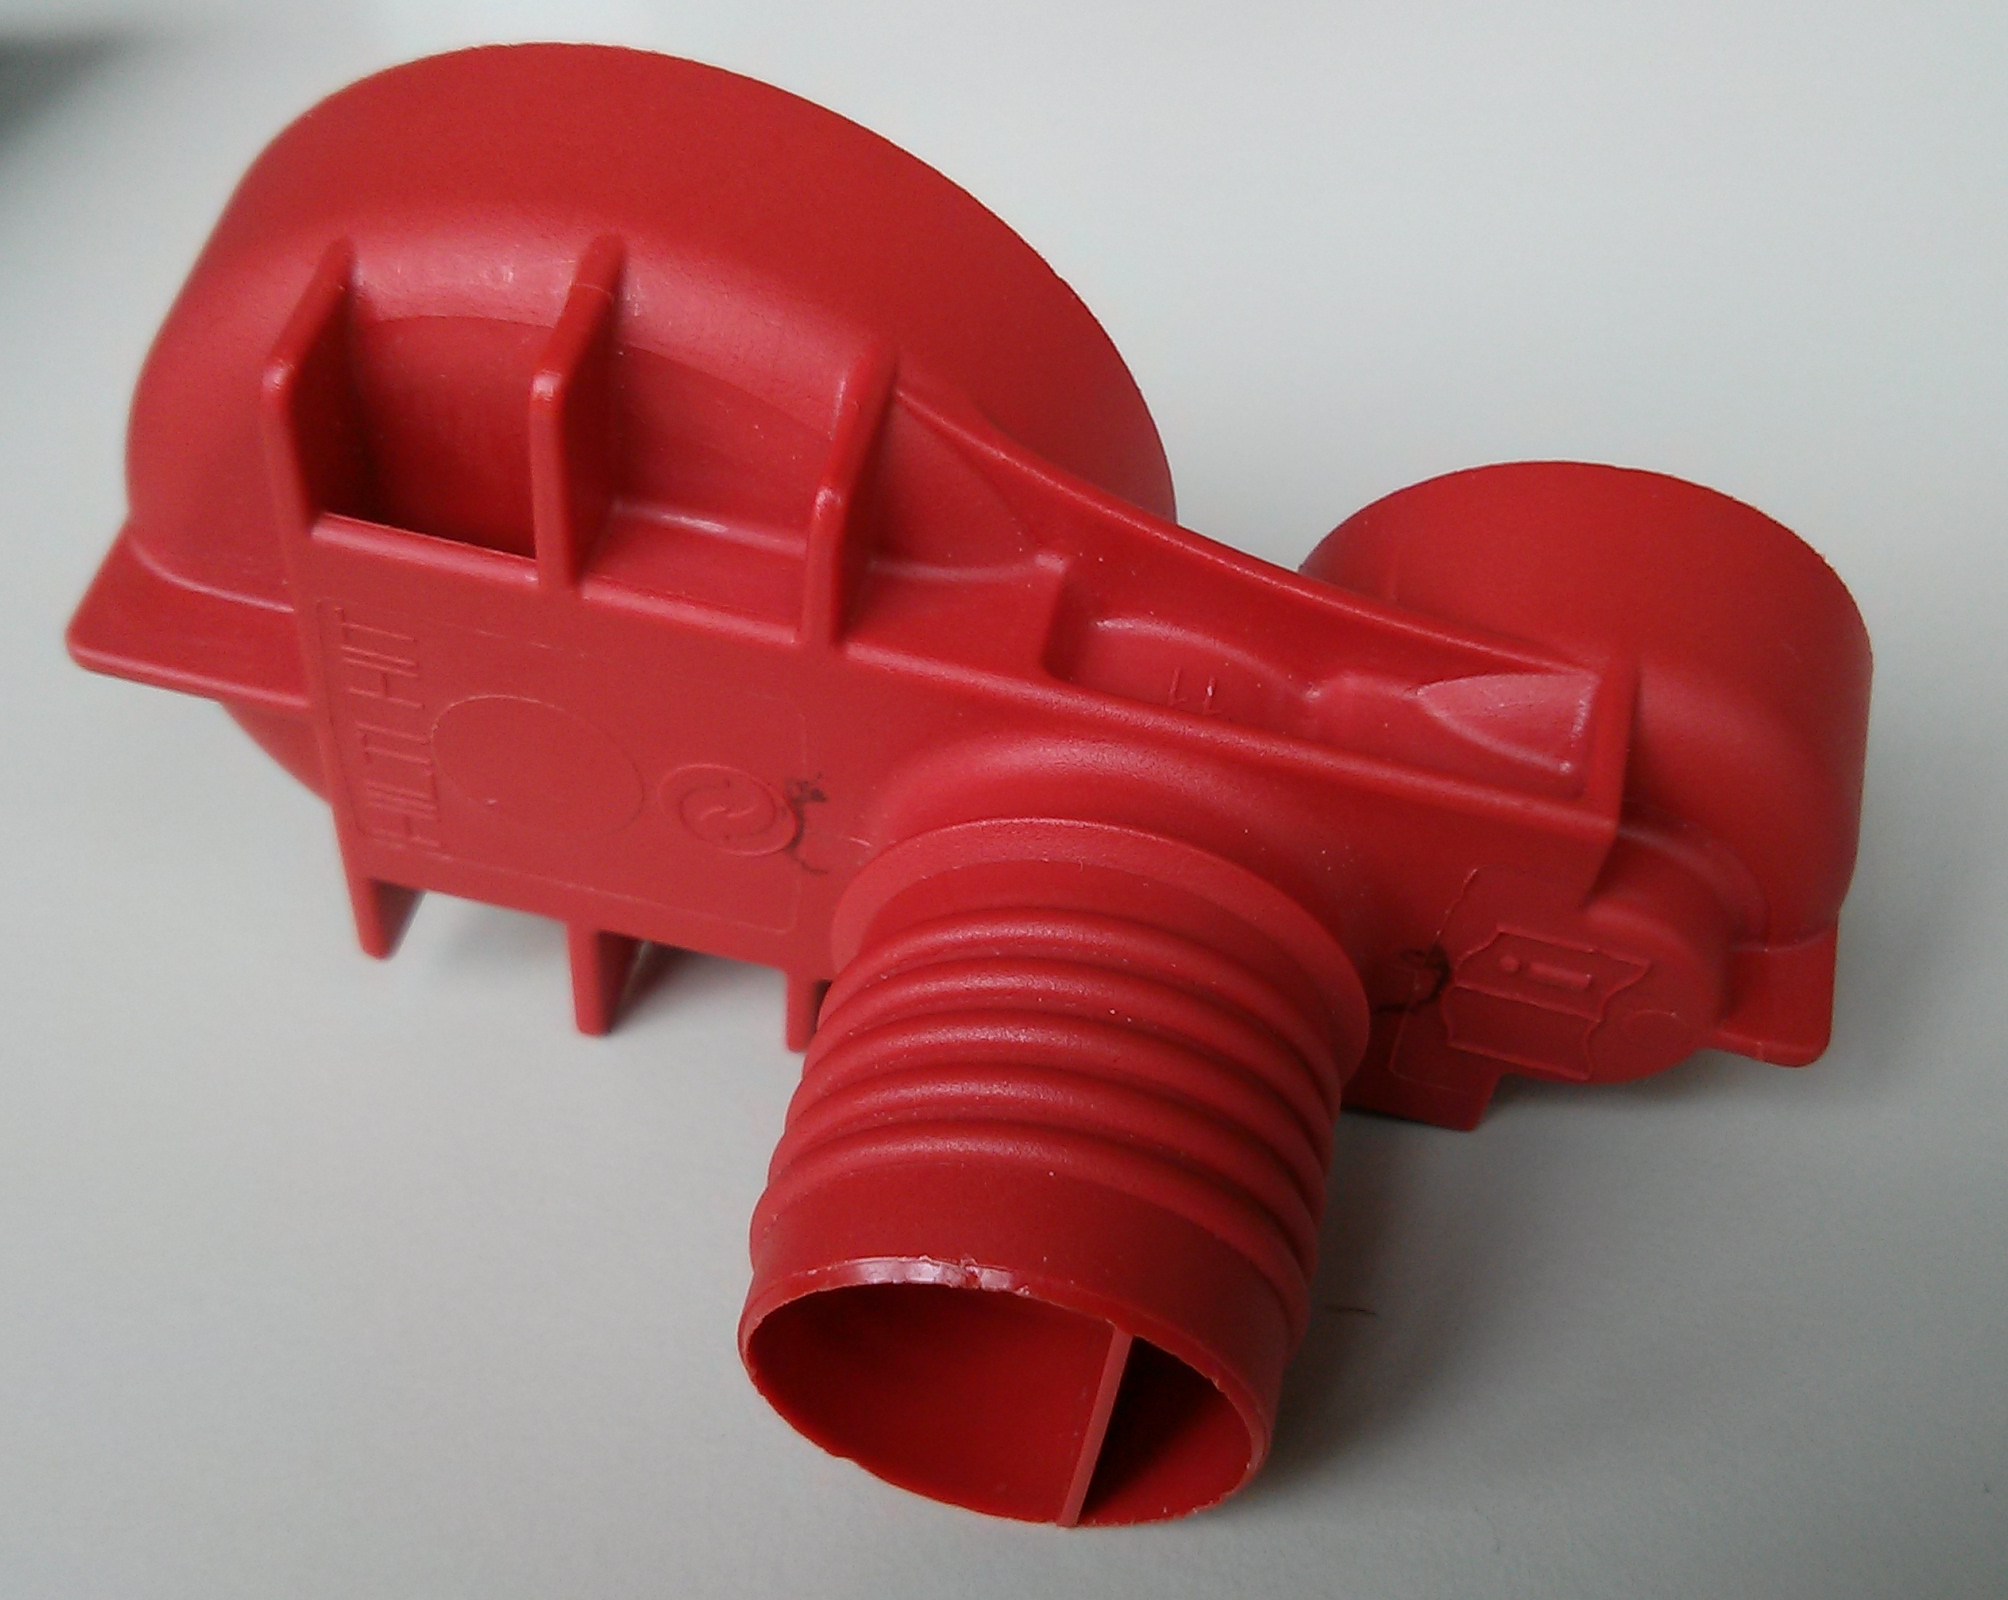
\includegraphics[width=0.2\textwidth]{figures/Mischeraufsatz.png}
        \label{fig:Mischer:subA}
    }
    \subfloat[Mischer HIT-RE-M]{
    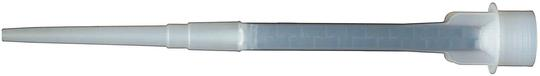
\includegraphics[width=0.67\textwidth]{figures/Mischer.jpg}
        \label{fig:Mischer:subB}
    }
    \caption{Das Mischermodell HIT-RE-M, in dem die Mörtel nach dem Auspressen gemischt werden.}
    \label{fig:Mischer}
\end{figure}
%
Dieser Mischer kann jeweils nur einmal verwendet werden, weil der Mörtel ab dem Zeitpunkt des Mischens beginnt auszuhärten und so den Mischer verstopft, sobald das Auspressen gestoppt wird. Es ist deshalb im Interesse des Verbrauchers, dass der Mischer im Erwerb sehr preiswert ist. Trotzdem soll er die Komponenten möglichst gut mischen, da dies entscheidend für die maximale Zuglast der Dübel ist.

Diese Ansprüche an das Gerät und den Mischer erfordern ein hohes Mass an Verständnis für die Vorgänge während dem Auspressen, weshalb sie in der Forschungsabteilung von Hilti ständig weiter vermessen, simuliert und verbessert werden.
%
\subsection{Messaufbau}
Das für die Mörtel verwendete Auspressgerät besteht zum grössten Teil aus Kunststoff. Da dieser selber elastische Eigenschaften besitzt, ist es sehr schwierig die viskoelastischen Eigenschaften eines Fluides zu bestimmen, das durch das Gerät fliesst.\\
Um einen Einfluss des Gerätes auf das Fluid auszuschliessen, wurde deshalb die Geometrie des Auspressgerätes in einer sogenannten Funktionsersatzprüfung (FEP) aus Metall nachgebaut. In Abbildung \ref{fig:FEP} sind Bilder dieser FEP zu sehen, in \ref{fig:FEP_schema} ist der Aufbau schematisch dargestellt.
%
\begin{figure}
    \centering
    \subfloat[Metallnachbau]{
        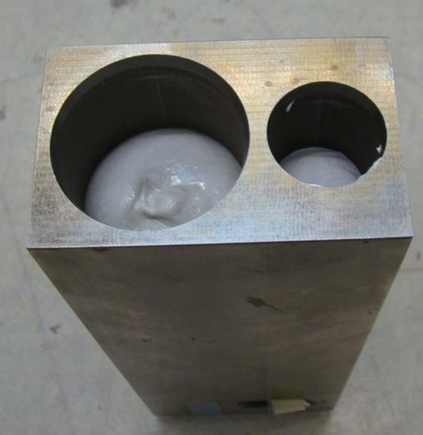
\includegraphics[width=0.31\textwidth]{figures/FEP_1.png}
        \label{fig:FEP:subA}
    }
    \subfloat[mit Mörtel gefüllt]{
        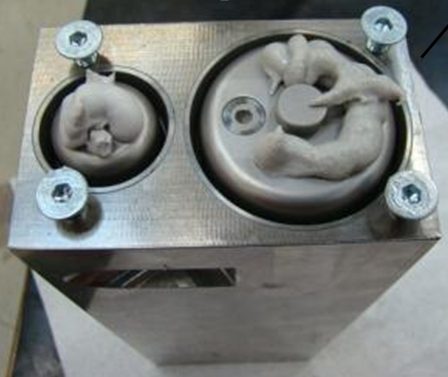
\includegraphics[width=0.31\textwidth]{figures/FEP_2.png}
        \label{fig:FEP:subB}
    } 
    \subfloat[Übergang zwischen Kolben und Mischer]{
        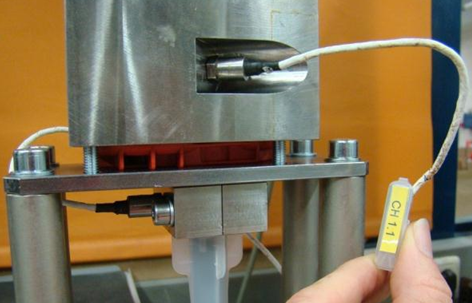
\includegraphics[width=0.31\textwidth]{figures/FEP_3.png}
        \label{fig:FEP:subC}
    }
    \caption{Der Messaufbau für das Auspressgerät.\\In Abbildung \subref{fig:FEP:subA} ist der Nachbau der Geometrie aus Metall zu sehen, der in \subref{fig:FEP:subB} mit Mörtel befüllt worden ist.\\
    Dieser Mörtel wird dann von einem Kolben durch eine Blende in den Mischer gepresst, der Übergang ist in \subref{fig:FEP:subC} zu sehen.}
    \label{fig:FEP}
\end{figure}
\todo{Bilder gleich gross}
%
\begin{figure}
    \centering
    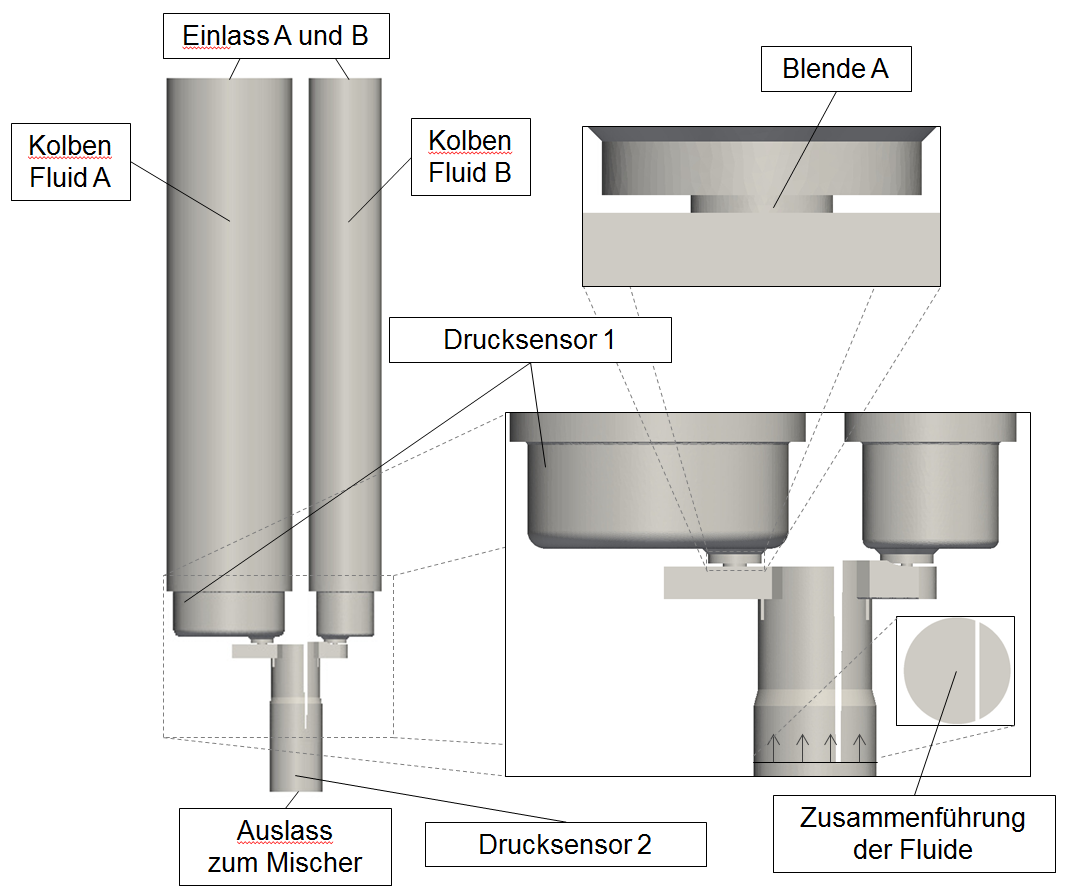
\includegraphics[width=\textwidth]{figures/FEP_Schema.png}
    \caption{Schematische Zeichnung der Funktionsersatzprüfung. Zu sehen sind die Kolbenwege der beiden Fluide,
    die Drucksensoren 1 und 2 und die Blende, deren Durchmesser variiert werden kann.}
    \label{fig:FEP_schema}
\end{figure}

Bei der Messung wird der Mörtel wird in die Metallröhre eingefüllt und dann von einem Kolben nach unten gedrückt. Beim Übergang zwischen FEP und Mischer ist auf jeder Seite eine auswechselbare Blende eingebaut, die den Durchmesser der engsten Stelle bestimmt durch die das Fluid fliessen muss. Danach kommen die beiden Ströme zusammen und werden in den Mischer geleitet.

Die variablen Grössen bei der Versuchsausführung sind dabei die Kolbengeschwindigkeit (und damit der Volumenstrom), die Grösse der eingelegten Blenden die de und der Typ des verwendeten Mörtels. In der Praxis sind dabei auf den zwei Seiten jeweils die A und die B Komponente des Mörtels, in der FEP wurde, um den Vergleich mit den Simulationen einfach zu machen, jeweils nur ein Typ Mörtel eingesetzt.

Gemessen wird jeweils vor dem Durchströmen der Blende und vor dem Mischereingang (Drucksensor 1 und 2 in Abbildung \ref{fig:FEP_schema}) der Druckunterschied zum Umgebungsdruck und die Kraft, die für das Runterdrücken der Kolben notwendig ist.
%
\subsection{Simulation}
Durch den Vergleich der gemachten Messungen mit Simulationen sollen Aussagen über die Verlässlichkeit der verwendeten Modelle gemacht werden können.\\
Dazu wurde die Geometrie der FEP und des Mischers virtuell nach gebaut und vernetzt. Dabei wurde darauf geachtet, dass die kritischen Regionen wie zum Beispiel die Blende in der FEP besonders fein vernetzt ist, während Regionen in denen erwartungsgemea;ss keine grosse Veränderung in den Variablen zu erwarten ist nur grob vernetzt sind. Ein Beispiel ist in Abbildung \ref{fig:FEP_Gitter} und \ref{fig:Mischer_Gitter} zu sehen.
%
\begin{figure}
    \centering
    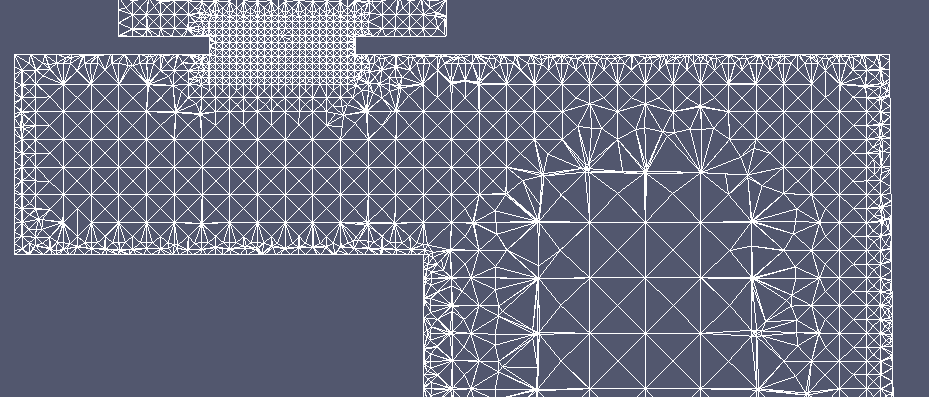
\includegraphics[width=\textwidth]{figures/FEP_Gitter1.PNG}
    \caption{Ein Ausschnitt des verwendeten Gitters für die FEP.\\
    Zu sehen ist oben links die Blende, die sehr fein aufgelöst ist. Nach unten wird das Netz wieder gröber, da die erwartete Änderung in $\u$ und $p$ kleiner ist.}
    \label{fig:FEP_Gitter}
\end{figure}
%
\begin{figure}
    \centering
    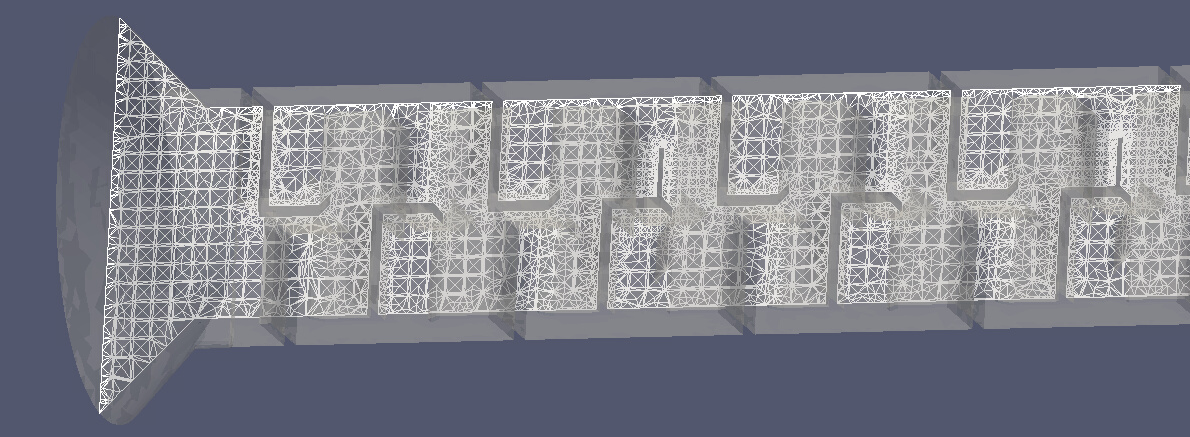
\includegraphics[width=\textwidth]{figures/Mischer_Gitter1.PNG}
    \caption{Ein Ausschnitt des verwendeten Gitters für den Mischer.\\
    Die Geometrie ist dabei transparent hellgrau dargestellt um den Ort des gezeigten Schnittes durch das Netz zu verdeutlichen.}
    \label{fig:Mischer_Gitter}
\end{figure}
%

Simuliert wurde mit den Lösern \codeemph{simpleFoam} und \codeemph{viscoelasticFluidFoam}. Dabei wurde stets eine steady state Lösung angestrebt bei der die Geschwindigkeit an den Einlässen vorgegeben wurde und dann gewartet wurde bis sich ein konstanter Gegendruck ausgebildet hatte. Das setzt voraus, dass der Einfluss des Kolbens mit einer konstanten Anströmung gleichgesetzt werden kann, was natürlich nur bei ausreichendem Abstand zwischen Kolben und Blende hinreichend genau stimmt.

Die berechneten Felder waren bei \codeemph{simpleFoam} die Geschwindigkeit $\u$ und der Druck $p$. Als Randbedingung wurde für $\u$ beim Einlass ein konstanter Wert, beim Auslass ein Null-Gradient und an den Wänden eine no-slip Bedingung vorgegeben. Der Druck $p$ wurde am Einlass auf Null (oder Umgebungsdruck) gesetzt und an allen anderen Boundaries ein Null-Gradient vorgegeben.\\
Für die Startlösung wurde wann immer möglich die Werte einer früheren Rechnung genommen. Dadurch kann die Konvergenzzeit drastisch verringert werden. \\
Falls für ein Netz keine alte Startwerte existierten, wurden alle Werte von $p$ und $\u$ im inneren auf Null gesetzt. Das ist vor allem für den Mischer eine eher schlechte Anfangsbedingung, weshalb hier nur Konvergenz erreicht werden konnte wenn die Relaxationsparameter hinreichend klein gewählt wurden.\\
Die Viskosität $\eta$ ist direkt abhängig von $\u$ und musste deshalb bei Start- oder Randbedingungen nicht berücksichtigt werden.

\codeemph{viscoelasticFluidFoam} arbeitet mit den drei Feldern Geschwindigkeit $\u$, Druck $\p$ und Schubspannungstensor $\tau$. Start- und Randbedingungen für $\u$ und $p$ wurden gleich wie beim Löser \codeemph{simpleFoam} behandelt, bei $\tau$ wurde am Einlass ein konstanter Wert von Null vorgegeben, an Wänden und beim Auslass wurde der Gradient auf Null gesetzt.
%
\subsection{Resultate}
\begin{todocontent}
    \1 Resultat Simulation (Bilder)
    \1 Druckvergleich
    \1 Einfluss Viskoelastizitaet
\end{todocontent}
